\documentclass[../main.tex]{subfiles}
\graphicspath{{\subfix{../images/}}}

\begin{document}

\subsection{\textbf{CDC}}

\noindent \textbf{Before moving to FastCDC:}  \\
The main design space that we explored was the chunk size that gets set by the modulus value. Initially this value was set to 1024 but we had to eventually increase this to 4096. A smaller chunk size would imply more deduplication but the compression and overall throughput increases with larger chunks. As mentioned in the project handout, we wanted to chunk with at least a size of 4096 bytes. Another thing that drastically helped improve our CDC throughput was pre calculating powers of 3 (which was our chosen PRIME) and storing them in a local buffer. Since the hash calculation was using powers of 3 up to 17 (this was based on our WIN\_SIZE used for the hash) repetitively for each iteration, we decided to pre-calculate these and store them in an array from which they can be read for hash calculations. This made our CDC significantly quicker. \\
\newline
\textbf{After moving to FastCDC:}  \\
To further optimize our CDC, we changed to FastCDC which used the GEAR hash and skipped sub-minimum chunk cut-points. Fast CDC theorizes that some of the hash calculations can be skipped when defining chunk boundaries in favor of a low probability that a chunk will occur at a position less than the desired average chunk size. To explain this let’s consider that we want chunks of size 4096, now the FastCDC says that the probability of drawing a chunk boundary at say 1024 (defined as the minimum chunk size) is very low, and hence we can skip hash calculation until the first 1024 bytes in a chunk. This drastically reduces the latency of CDC while efficiently drawing good chunk boundaries. \\
\newline
Now the GEAR hash consists of essentially a lookup table of 256 values and the hash value for a certain character is the value stored at the index represented by the ASCII value of that character. This means that the hash calculation only requires an array lookup. This along with the skipping of hash calculations, made our final CDC implementation much faster as opposed to regular CDC.\\

\vspace{1cm}

\noindent \textbf{Data: Test Case - Franklin Text File (File Size: 399054 B)}

\begin{table}[H]
    \centering
    \begin{tabular}{|c|c|c|c|c|c|} \hline 
         Chunk&  Total&  CDC &  SHA &  LZW &  DEDUP \\ 
         Size& Throughput&  Throughput&  Throughput&  Throughput&  Throughput \\
         & (Mb/s)&  (Mb/s)&  (Mb/s)&  (Mb/s)&  (Mb/s) \\ \hline
         2048&  58.4843&  1781.58&  551.707&  79.0904&  5561.34 \\ \hline 
         4096&  67.443&  1178.01&  713.09&  92.6546&  8704.41\\ \hline 
         8192&  72.8656&  1000.7&  851.229&  100.217&  13057 \\ \hline
    \end{tabular}
    \caption{Chunk Size Versus Throughput - Franklin}
    \label{tab:chunk_graph}
\end{table}

\vspace{1cm}

\begin{table}[H]
    \centering
    \begin{tabular}{|c|c|c|c|} \hline 
         Chunk&  Contributed & Contributed& Compression\\
         Size&  DEDUP (B)& LZW (B)& Ratio\\ \hline
         2048&  0&  327310& 0.82\\ \hline 
         4096&  0&  291731& 0.73\\ \hline 
         8192&  0&  259191& 0.65\\ \hline
    \end{tabular}
    \caption{Chunk Size Versus Compression Ratio - Franklin}
    \label{tab:chunk_comp}
\end{table}

\vspace{0.5cm}

\noindent The graph below was generated by using the data points that we have and extrapolating them using the power rule, i.e., $y=Ax^B$. This enabled us to estimate the values of throughput and compression ratios for values of chunk size ranging from 256 to 65536, and then plot them. \\

\begin{figure}[H]
    \centering
    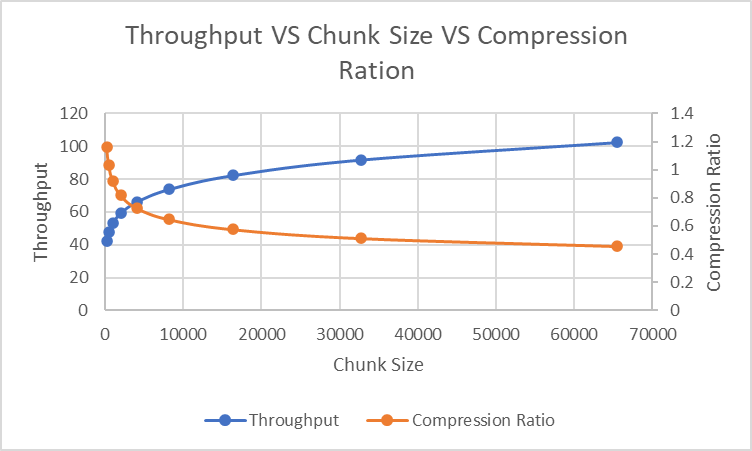
\includegraphics[width=0.7\linewidth]{Images/image19.png}
    \caption{Chunk Size VS Throughput VS Compression Ratio Graph}
    \label{fig:chunk_comp_graph}
\end{figure}

\vspace{0.5cm}

\noindent \textbf{Data: Test Case - vmlinuz\_small.tar (File Size: 399054 B)}

\begin{table}[H]
    \centering
    \begin{tabular}{|c|c|c|c|c|c|} \hline 
         Chunk&  Total&  CDC &  SHA &  LZW &  DEDUP \\ 
         Size& Throughput&  Throughput&  Throughput&  Throughput&  Throughput \\
         & (Mb/s)&  (Mb/s)&  (Mb/s)&  (Mb/s)&  (Mb/s) \\ \hline
         2048&  73.3759&  1639.94&  593.419&  89.3484&  10673.8\\ \hline 
         4096&  87.4704&  1099.73&  776.749&  109.426&  16190.4\\ \hline 
         8192&  94.3199&  965.239&  911.699&  119.165&   20780\\ \hline
    \end{tabular}
    \caption{Chunk Size Versus Throughput - vmlinuz\_small}
    \label{tab:chunk_graph_2}
\end{table}

\begin{table}[H]
    \centering
    \begin{tabular}{|c|c|c|c|} \hline 
         Chunk&  Contributed & Contributed& Compression\\
         Size&  DEDUP (B)& LZW (B)& Ratio\\ \hline
         2048&  768&  643& 0.004\\ \hline 
         4096&  380&  734& 0.003\\ \hline 
         8192&  184&  938& 0.003\\ \hline
    \end{tabular}
    \caption{Chunk Size Versus Compression Ratio - vmlinuz\_small}
    \label{tab:chunk_comp_2}
\end{table}

\subsection{\textbf{SHA 256}}
Initially we were using a software implementation from the \href{https://github.com/james-ben/mpsoc-crypto}{mpsoc-crypto} library provided in the
project handout. To optimize this further, we moved the SHA implementation onto the ARM NEON cores since this was an effective method of exploiting
parallelism. \\
\newline
For our final implementation, we adapted the NEON intrinsics version of the implementation. The \href{https://github.com/james-ben/mpsoc-crypto}{mpsoc
-crypto} library provided in the project handout was used for this. This uses the SHA cryptographic intrinsics as well as the NEON intrinsics which
gives us significant speedup for the SHA since it uses 8 vector lanes.

\subsection{\textbf{LZW Kernel}}
We tried to exploit various design axes while trying to optimize the LZW kernel. We started by removing the for loop from the associative memory lookup (assoc\_lookup) function and replaced these with bit shifting and manipulation operations. Since, ‘for’ loops are computation intensive, this change helped us decrease the latency significantly.  Additionally, the main LZW loop initially consisted of a while loop. We changed this to a for loop since they are much faster and to help Vitis HLS know that the number of iterations are already known. We pipelined these loops to help decrease the II and make it more efficient. We also implemented	load-store-compute which enabled us to stream data across these functions in the kernel.\\ \\
We were also getting many hash collisions with the original hash function. To counter this, we also adapted the murmur hash in our LZW kernel implementation to reduce the hash collisions. This also allowed us to decrease the size of our hash table which resulted in reduced lookup times. 
As mentioned in the previous milestones, we also made use of 2 buckets instead of the one since we were getting multiple hash collisions for bigger binary files. This meant that each index was associated with 2 key-value pairs instead of just one. As a result of which, the associative memory would only come into use when 2 keys have already been previously hashed to the same index and entered into the main hash table. This decreased the entries in our associative memory significantly.\\ \\
To reduce the number of calls to the kernel and minimize the data transfer overhead we batched all the chunks in a 16KB buffer and sent that as a whole to the kernel in the kernel it would iterate over all the chunks and compute LZW. This gave us a huge speedup in comparison to calling the kernel in a loop based on the output from DEDUP. Once the data was received back from the kernel we would use the output from DEDUP to decide what to write into the compressed file.\\ \\
Apart from that to minimize the kernel overhead we reduced the amount of input arguments required. Firstly, the chunk\_indices array for the batched chunks that needed to be sent to LZW consisted of its first element being set to the length of the array; this way we avoided sending another parameter to the kernel and decreasing the setup time. Similarly for the out\_packet\_lengths argument of the kernel which populated the length of the encoded LZW chunks had its first element signify if insertion into the associative memory had failed. This helped us further reduce the data transfer time. 
As described previously in section III under “Challenges and Debugging”, we noticed that with binary files the code value in LZW exceeded 4096, which was the configuration for our hash table lookup and bit packing. Due to this we decided to move to a 13-bit packing routine and modified the hash table to support 13-bit values, and updated the size of the key accordingly. This helped us mitigate the issue of the code exceeding 4096 and ensured that our design would be stable and functional for our configured chunk size.\\ \\
Another optimization that we tried was moving the bit packing inside the kernel and producing the bit-packed output for the batched chunks. We thought that this would give us a significant speedup, instead it slowed down our kernel and the overall performance of the application took a hit. We tried to optimize the bit-packing in Vitis by pipelining and unrolling wherever possible, but it didn’t help. Due to this we decided to move the bit-packing routine outside the kernel and back onto the ARM processor.\\ \\
Finally, another optimization that we tried was to reduce the number of parameters sent to our compression\_pipeline function, since the OpenCL buffers were set up in main and then they were passed to the compression\_pipeline function along with their host mapped buffers. Apart from this the function took in a lot of other parameters like the OpenCL command queue, the kernel, the file pointer to write into the file, etc. Hence to minimize the amount of arguments, we tried to wrap the OpenCL buffers and their host counterparts into a struct and tried to pass a pointer to that struct, but when we did that we weren’t able to properly retrieve data back into our buffer from the kernel and decided to get rid of it, in interest of complete functionality.


\end{document}